\documentclass[a4paper,9pt]{extarticle}

\title{cheat sheet}
\date{2017-09-16}

\usepackage{pew}
\setcounter{section}{1}

\begin{document}
\begin{multicols*}{2}
\section{Introduction}
\subsection{Events [2.2]}
\begin{enumerate}[label=\bfseries (\arabic*)] \itemsep0pt \parskip0pt
    \item The result $u_1$ of a random trial is called \textbf{outcome}.
    \item The set of all possible outcomes is called \textbf{sample space $\Omega$}.
    \item A collection of outcomes $A$ is called \textbf{event}.
\end{enumerate}

Thus an event is a subset of the sample space (or possibly the whole sample space).

The events $A_1, ..., A_n$ are said to be \textbf{mutually exclusive} (or \textbf{mutually disjoint}) if all pairs $A_i, A_j$ are exclusive; that is, if it is impossible that two or more of these events take place at the same time.

\subsection{Sample spaces [2.2]}
If the number of outcomes is finite or denumerably infinite, $\Omega$ is said to be a \textbf{discrete sample space}. More particularly, if the number is finite, $\Omega$ is said to be a \textbf{finite sample space}.

If the number of outcomes is neither finite nor denumerably infinite, $\Omega$ is said to be a \textbf{continuous sample space}.

\subsection{Kolmogorov's System of Axioms [2.3]}
The following axioms for the probabilities $P(\cdot)$ should be fulfilled:
\begin{enumerate}[label=\bfseries A\arabic*.] \itemsep0pt \parskip0pt
    \item If $A$ is any event, then $0 \leq P(A) \leq 1$.
    \item If $\Omega$ is the entire sample space, then $P(\Omega) = 1$.
    \item ("Addition Formula"). If $A$ and $B$ are mutually exclusive events, then $P(A \cup B) = P(A) + P(B)$.
\end{enumerate}

The sample space $\Omega$ and the probabilities $P(\cdot)$ together constitute a \textbf{probability space}.

\subsection{Results from Kolmogorov's system [2.3]}
\textbf{Complement Theorem}
\begin{equation}
    P(A*) = 1 - P(A)
\end{equation}
\begin{equation}
    P(\varnothing) = 0
\end{equation}

\noindent \textbf{Addition Theorem}
\begin{equation}
    \begin{split}
        P(A \cup B) & = P(A) + P(B) + P(A \cap B) \\
        P(A \cup B \cup C) & = P(A) + P(B) + P(C) - P(A \cap B) \\
        & - P(A \cap C) - P(B \cap C) + P(A \cap B \cap C)
    \end{split}
\end{equation}

\noindent \textbf{Boole's Inequality}
\begin{equation}
    \begin{split}
        P(A \cup B) & \leq P(A) + P(B) \\
        P(A \cup B \cup C) & \leq P(A) + P(B \cup C) \\
        & \leq P(A) + P(B) + P(C)
    \end{split}
\end{equation}

\subsection{Probabilities in Discrete Sample Spaces [2.4]}
\begin{equation} \label{2.4.1}
    P(u_i) = 1/m \quad (i = 1, 2, \ldots, m)
\end{equation}
If (\ref{2.4.1}), we have a \textbf{uniform probability distribution}. \\

An event $A$ with $g$ outcomes, has \textbf{$g$ favourable cases}. That means there are \textbf{$m$ possible cases} in $\Omega$. We then determine $P(A)$ from the addition formula by adding the probabilities $m$ of the $g$ outcomes. Hence,
\begin{equation}
    P(A) = g/m
\end{equation}

\subsection{Urn model [2.4]}
Let's examine the probability of drawing exactly $k$ white balls from an urn containing $a$ white and $b$ black balls, $n$ balls are drawn.

If one ball at a time is drawn at random without returning it to the urn, the drawings are said to be made \textbf{without replacement}. The probability is then:
\begin{equation}
    \frac{\binom{a}{k} \binom{b}{n-k}}{\binom{a + b}{n}}
\end{equation}

If one ball at a time is drawn at random and is returned before the next ball is drawn, the drawings are said to be made \textbf{with replacement}. The probability is then:
\begin{equation}
    \binom{n}{k} p^k q^{n-k}
\end{equation}
where
\begin{equation}
    p = \frac{a}{a+b}, \quad q = 1 - p = \frac{b}{a+b}
\end{equation}

\subsection{Conditional Probability [2.5]}
\begin{equation}
    \begin{split}
        P(B|A) & = \frac{P(A \cap B)}{P(A)} \\
        P(A \cap B) & = P(A) P(B|A) = P(B) P(A|B)
    \end{split}
\end{equation}

is called the \textbf{conditional probability of B given A}.
{\centering 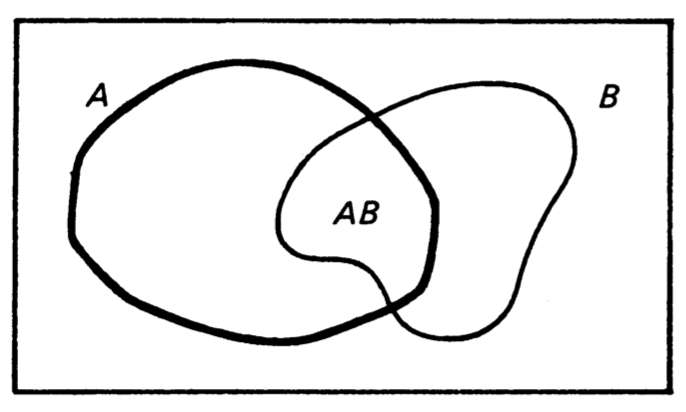
\includegraphics[scale=0.25]{conditional-probability} \par}

From this we can derive the \textbf{Total Probability Theorem}. If the events $H_1, H_2, \dots , H_n$ are mutually exclusive, have positive probabilities, and together fill $\Omega$ completely, any event $A$ satisfies the formula:
\begin{equation}
    P(A) = \sum_{i=1}^n P(H_i) P(A|H_i)
\end{equation}
{\centering 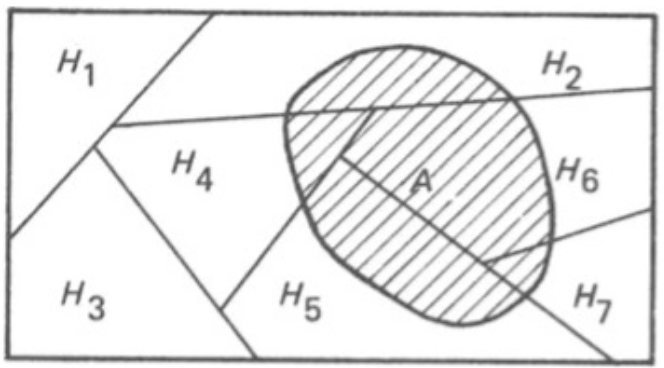
\includegraphics[scale=0.25]{total-probability} \par}

And \textbf{Bayes' Theorem}:
\begin{equation}
    P(H_i|A) = \frac{P(H_i) P(A|H_i)}{\sum_{j=1}^n P(H_j) P(A|H_j)}
\end{equation}

\subsection{Independent Events [2.6]}
\begin{equation} \label{2.6.1}
    P(A \cap B) = P(A) P(B),
\end{equation}
If (\ref{2.6.1}), then $A$ and $B$ are said to be \textbf{independent events}. This can be extended to three events. Consequence:

If the events $A_1, A_2, \dots, A_n$ are independent and $P(A_i)=p_i$, then the probability that at least one of them occurs is equal to
\begin{equation}
    1 - (1 - p_1)(1 - p_2) \cdots (1 - p_n)
\end{equation}

If the events $A_i$ are independent and each one of them occurs with probability $p$, then the probability that at least one of them occurs is equal to $1 - (1 - p)^n$.

Two trials as \textbf{independent}, if the result of one does not affect, or is not affected by, the result of the other. An important special case is provided by \textbf{repeated trials}.

\subsection{Theorems in Combinatorics [2.7]}
Drawing $n$ elements from $N$:

\renewcommand{\arraystretch}{1.5}
\begin{tabulary}{1.0\textwidth}{r|c|c}
    & with replacement & without replacement \\ \hline
    order & $N^n$ & $N (N-1) \cdots (N-n+1)$ \\ \hline
    no order & $\binom{N+n-1}{n}$ & $\binom{N}{n}$ \\
\end{tabulary}

\rule{0pt}{0.5em}
\renewcommand{\arraystretch}{1}

The \textbf{multiplication principle} states: If choice 1 can be performed in $a_1$ ways and choice 2 in $a_2$ ways, then there are $a_1 a_2$ ways to perform both choices. In the case of three choices, the number of ways is $a_1 a_2 a_3$, and so on.

\section{One-Dimensional Random Variables}
\subsection{General Description of Random Variables [3.2]}
A random variable ($rv$) is a function defined on a sample space.

\subsection{Distribution Function [3.3]}
$F_X(x) = P(X  \leq x)$ is called the (cumulative) distribution function of the $rv$ $X$.

{\centering 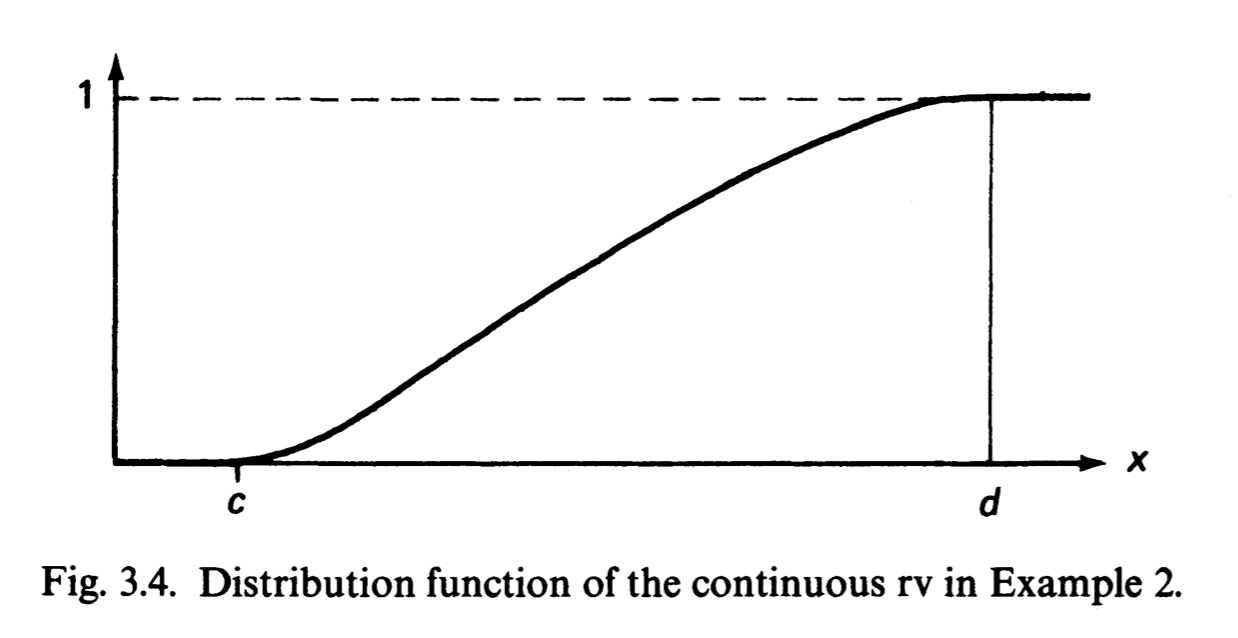
\includegraphics[scale=0.25]{distribution-function} \par}

\textbf{Theorem 1.} The distribution function $F_X(x)$ of a $rv$ $X$ has the properties:
\begin{enumerate}[label=\bfseries \arabic*.]
    \item $\lim_{x \to -\infty} F_X(x) = 0$
    \item $\lim_{x \to \infty} F_X(x) = 1$
    \item $F_X(x)$ is a nondecreasing function of $x$
    \item $F_X(x)$ is continuous from the right for any $x$
\end{enumerate}

\textbf{Theorem 2.} If $a \leq b$, then
\begin{equation} \label{3.3.1}
    F_X(b) - F_X(a) = P(a < X \leq b)
\end{equation}

\subsection{Discrete Random Variables [3.4]}
A random variable is \textbf{discrete} if it can assume a finite or a denumerably infinite number of different values.

The quantities $p_X(k) (k = 0, 1, ...)$ are jointly called the \textbf{probability function} of the $rv$ $X$.

\subsection{Discrete Distributions [3.5]}
\begin{enumerate}[label=\bfseries (\alph*)]
    \item \textbf{One-Point}. $p_X(a) = 1$.
    \item \textbf{Two-Point}. $p_X(a) = p;$ $p_X(b) = q$.
    \item \textbf{Uniform}. $p_X(k) = \frac{1}{m}, \quad k = 1,2, ..., m$.
    \item \textbf{Geometric}. $p_X(k) = q^k p, \quad q = 1-p, \quad k = 0,1, ...$.
    \item \textbf{Binomial}. $p_X(k) = \binom{n}{k} p^k q^{n-k}, \quad k = 0,1, ..., n$.
    \item \textbf{Hypergeometric}. $p_X(k) = \binom{a}{k} \binom{b}{n-k} / \binom{a + b}{n}, \\ 0 \leq k \leq a, 0 \leq n - k  \leq b$
    \item \textbf{Poisson}. $p_X(a) = e^{-m} m^k / k!, \quad k = 0, 1, ...$.
\end{enumerate}

\subsection{Density function [3.6]}
If a function $f_X(x)$ exists, such that
\begin{equation} \label{3.6.1}
    F_X(b) - \int_{-\infty}^{x} f_X(t) dt
\end{equation} is valid, we say that $X$ is a \textbf{continuous} $rv$. The function $f_X(x)$ is called the \textbf{density function} of $X$.

The density function shows how the total probability mass of $1$ is distributed over the infinitely many $x$-values:
\begin{equation} \label{3.6.2}
    \int_{-\infty}^{\infty} f_X(t) dt = 1
\end{equation}


\textbf{Theorem 3.} At any point of continuity $x$ of $f_X(x)$:
\begin{equation} \label{3.6.3}
    F'_X(x) = f_X(x)
\end{equation}

Hence
\begin{equation}
    \begin{split}
        F_X(b) - F_X(a) & = \int_a^b f_X(t) dt \\
        P(a < X \leq b) & = \int_a^b f_X(t) dt \quad (a < b)
    \end{split}
\end{equation}

The solution $x = x_\alpha$ of the equation $F_X(x) = 1 - \alpha$
is called the \textbf{$\alpha$-quantile} (or fractile) of the $rv$ $X$.

{\centering 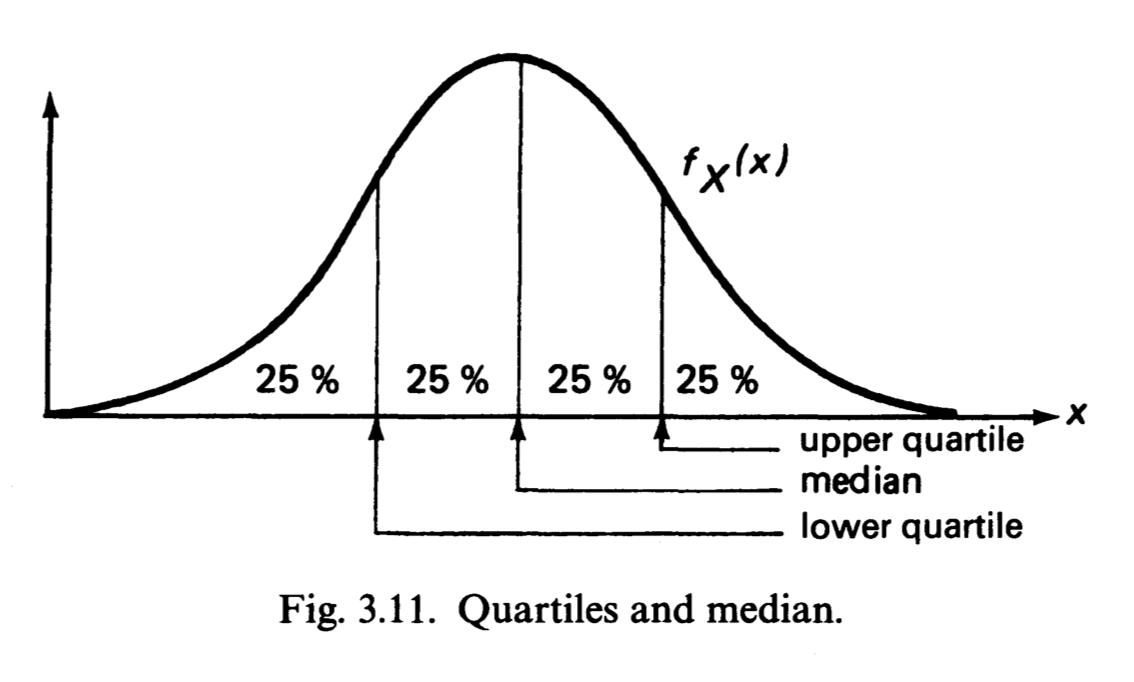
\includegraphics[scale=0.25]{quantile} \par}

\subsection{Continuous Distributions [3.7]}
\begin{enumerate}[label=\bfseries (\alph*)]
    \item \textbf{Uniform}. \begin{equation}
        f_X(x)=\begin{cases}
            1/(b-a) & \text{if $a < x < b$}\\
            0 & \text{otherwise}
        \end{cases}
    \end{equation}
    \item \textbf{Exponential}. \begin{equation}
        f_X(x)=\begin{cases}
            \frac{1}{m} e^{-x/m} & \text{if $x \geq 0$}\\
            0 & \text{if $x < 0$}
        \end{cases}
    \end{equation} where $m > 0$. Code name $X \sim Exp(m)$.
    \item \textbf{Normal}. $f_X(x) = \frac{1}{\sigma \sqrt{2 \pi}} e^{-(x-m)^2 / 2 \sigma^2} \quad (-\infty < x < \infty)$, where $m$ and $\sigma$ are given quantities $(\sigma > 0)$. Also called Gaussian. Code name $X \sim N(m, \sigma^2)$
    \item \textbf{Weibull?}
    \item \textbf{Gamma?}
\end{enumerate}

{\centering 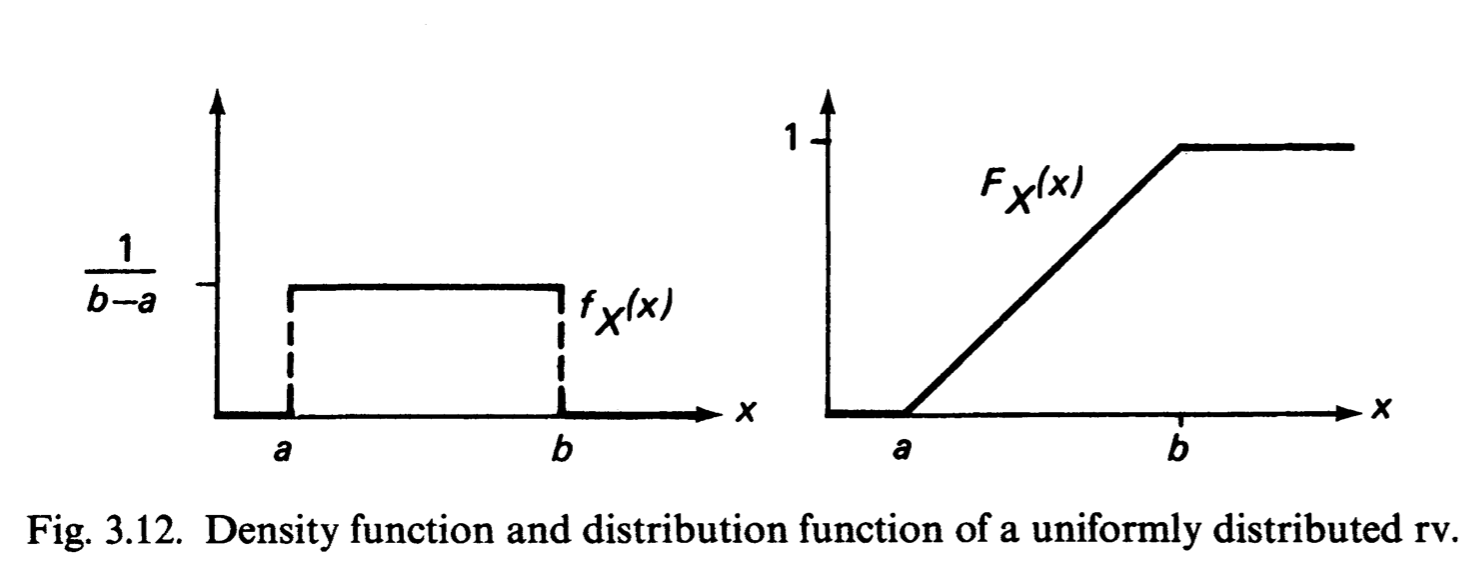
\includegraphics[scale=0.3]{continuous-uniform} \par}
{\centering 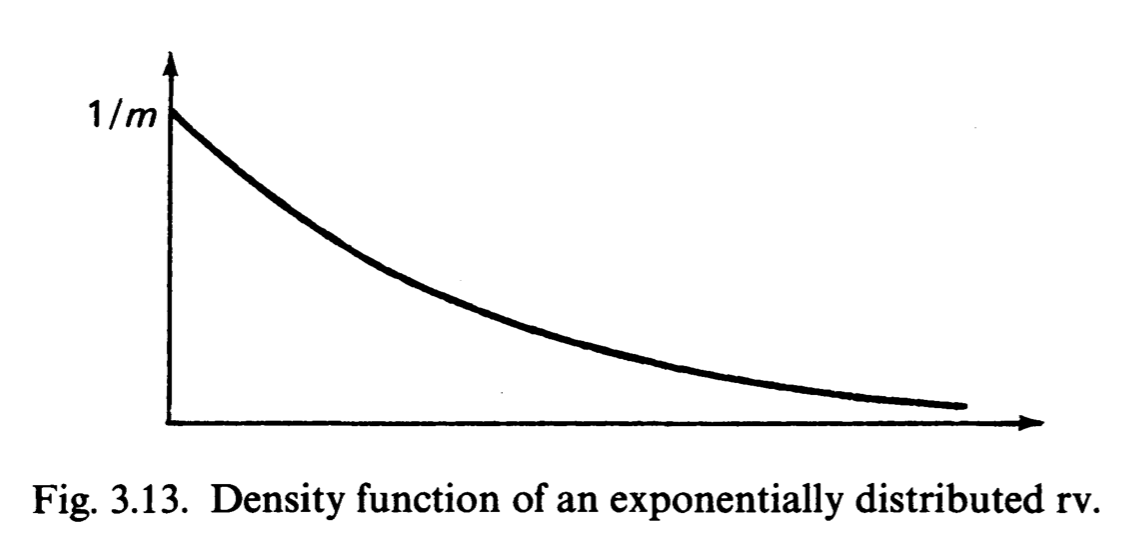
\includegraphics[scale=0.3]{continuous-exponential} \par}
{\centering 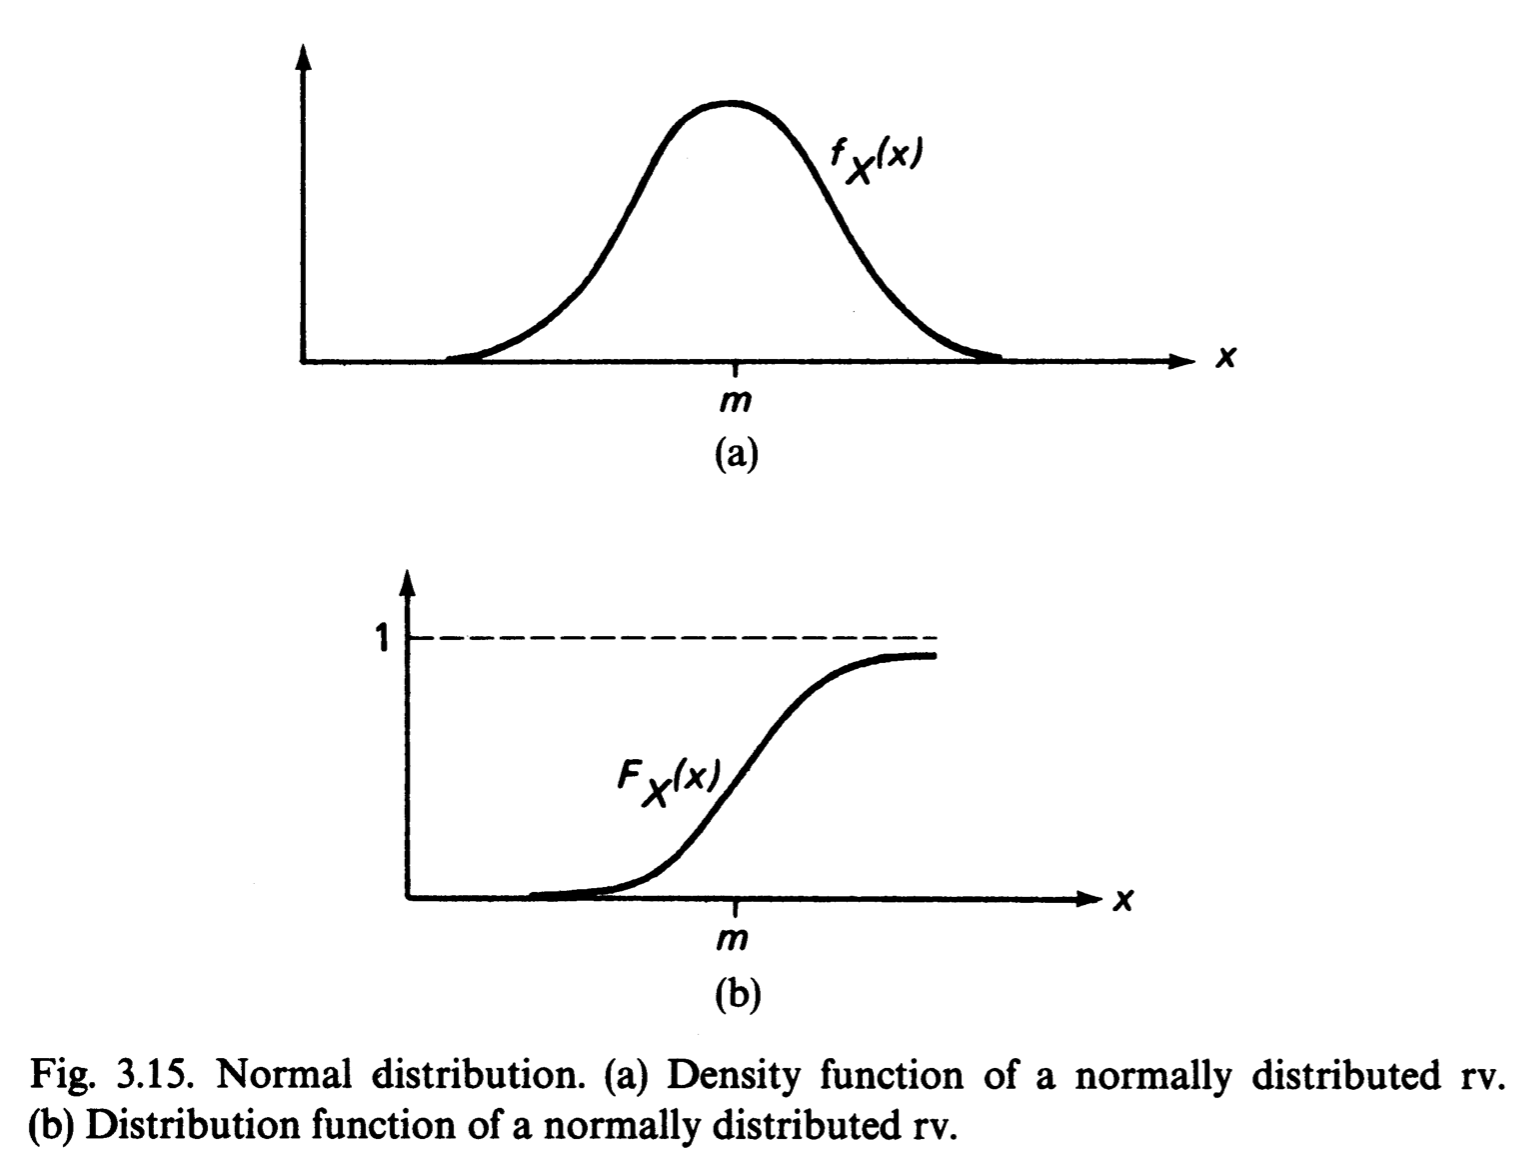
\includegraphics[scale=0.3]{continuous-normal} \par}

\section{Multidimensional Random Variables}
\subsection{Independent Random Variables [4.5]}
The $rv$'s $X$ and $Y$ are called \textbf{independent} if, for all $j$ and $k$ or $x$ and $y$, we have
\begin{equation}
    \begin{split}
        p_{X,Y}(j,k) & = p_X(j) p_Y(k) \quad (\text{discrete rv's}) \\
        f_{X,Y}(x,y) & = f_X(x) f_Y(y) \quad (\text{continuous rv's})
    \end{split}
\end{equation}

The following definition is equivalent: The $rv$'s $X$ and $Y$ are called independent if, for all $x$ and $y$, we have
\begin{equation}
    F_{X,Y}(x,y) = F_X(x) F_Y(y)
\end{equation}

\section{Functions of Random Variables [5.2]}
\subsection{A Single Function of a Random Variable}
Consider the $rv$ $Y = g(X)$ and find the distribution of $Y$. \textbf{Method:}

\begin{enumerate}[label=\bfseries (\arabic*)] \itemsep0pt \parskip0pt
    \item Determine the distribution function $F_Y(y)$ of $Y$: $F_Y(y) = P(g(x) \leq y) = ... = P(X \leq g'(x)) = F_X(g'(x))$.
    \item Obtain density funciton by differentiating the distribution function with respect to $y$.
\end{enumerate}

\subsection{Sums of Random Variables [5.3]}
The "addition" of two random variables $X$ and $Y$ is often called \textbf{convolution of the distributions of $X$ and $Y$}. The distribution function of $Z = X + Y$ is obtained by integrating the joint density funtion $f_{X,Y}(x,y)$ over the region $x + y \leq z$:
\begin{equation}
    F_Z(z) = \iint_{x + y \leq z} f_{X,Y}(x,y) dx dy
\end{equation}
or for independent $X$ and $Y$:
\begin{equation}
    F_Z(z) = \iint_{x + y \leq z} f_{X}(x) f_{Y}(y) dx dy
\end{equation}
which can be rewritten to the \textbf{convolution formula for independent continuous rv's}:
\begin{equation}
    F_Z(z) = \int_{-\infty}^{\infty} f_{X}(x) f_{Y}(z - x) dx
\end{equation}

\subsection{Largest Value and Smallest Value [5.4]}
\textbf{Larger of Two Values}
Set $Z = max(X, Y)$. $Z \leq z$ if and only if both $X \leq z$ and $Y \leq z$, hence
\begin{equation}
    F_Z(z) = P(Z \leq z) = P(X \leq z \wedge Y \leq z) = F_X(z) F_Y(z)
\end{equation}

\textbf{Smaller of Two Values}
Set $Z = min(X, Y)$. Since $Z > z$ if and only if both $X > z$ and $Y > z$,
\begin{equation}
    \begin{split}
        F_Z(z) & = P(Z \leq z) = 1 - P(Z > z) \\
        & = 1 - P(X > z \wedge Y > z) \\
        & = 1 - P(X > z) P(Y > z)
    \end{split}
\end{equation}
With $P(X > z) = 1 - P(X \leq z) = 1 - F_X(z)$, we find that:
\begin{equation}
    F_Z(z) = 1 - [1 - F_X(z)][1 - F_Y(z)]
\end{equation}

\subsection{Ratio of Random Variables [5.5]}
Determine the distribution of the rv $Z = X/Y$:
\begin{equation}
    F_Z(z) = P(X/Y \leq z) = P(X \leq Yz), \quad y \geq 0
\end{equation}

The distribution function is
\begin{equation}
    F_Z(z) = \int_0^{\infty} F_X(yz) f_Y(y) dy
\end{equation}

Whenever differentiation under the integral sign is permissible, we get the density function
\begin{equation}
    F_Z(z) = \int_0^{\infty} y f_X(yz) f_Y(y) dy
\end{equation}

\section{Expectations}
\subsection{Definition and Simple Properties [6.2]}
The \textbf{expectation} of the rv $X$ is defined by

\begin{equation}
    E(X) = \mu = \begin{cases}
        \sum_k k p_X(k) & \text{discrete rv} \\
        \int_{-\infty}^{\infty} x f_X(x) dx & \text{continuous rv}
    \end{cases}
\end{equation}

Instead of expectation we often use the term \textbf{mean}. The symbol $E(X)$ is often replaced by $m$, $m_X$ or some other symbol.

Analogously, the expectation of a function $Y = g(X)$ of a rv $X$:
\begin{equation}
    E(Y) = \begin{cases}
        \sum_k g(k) p_X(k) & \text{discrete rv} \\
        \int_{-\infty}^{\infty} g(x) f_X(x) dx & \text{continuous rv}
    \end{cases}
\end{equation}
and for $Z = g(X, Y$
\begin{equation}
    E(Z) = \begin{cases}
        \sum_{j,k} g(j,k) p_{X,Y}(j,k) & \text{discrete rv} \\
        \int_{-\infty}^{\infty} \int_{-\infty}^{\infty} g(x,y) f_{X,Y}(x,y) dx dy & \text{continuous rv}
    \end{cases}
\end{equation}

\textbf{Properties:}
\begin{enumerate}[label=\bfseries (\arabic*)] \itemsep0pt \parskip0pt
    \item $E$ is a linear operator: $E[g(X) + h(X)] = E[g(X)] + E[h(X)]$
    \item If $Y$ is a linear function $Y = a X + b$, it follows that $E(A X + b) = a E(X) + b$.
    \item The mean is a measure of location: If a constant $b$ is added to the rv, then $b$ is added to the mean.
\end{enumerate}

\subsection{Measures of Location and Dispersion [6.3]}
In order to give a complete description of a rv we use the distribution function or the probability function/density function. When such detailed knowledge is not required, we may use other measures which describe some property of the distribution. Of particular value are:

\subsubsection{Measures of Location}
The expectation $E(X)$ is a measure of location that shows where the mass is situated "on the average". Another measure is the \textbf{median}$x_{0.50}$, denoted by $\widetilde{m}$.

\subsubsection{Measures of Dispersion}
Since two rv's can have the same expectation with different distributions, the measure of location alone is not enough. Measures of dispersion include:

The \textbf{variance} $V(X)$ of the rv $X$ is defined by
\begin{equation}
    V(X) = E[(X - m)^2] = E(X^2) - [E(X)^2]
\end{equation}

Hence the variance is the expectation of the rv $Y = (X - m)^2$, where $m = E(X)$. This is sensible: If the distribution is concentrated around $m$, then $(X - m)^2$ assumes small values with large probability, and the variance is small. In particular, if the whole probability mass is concentrated at one single point, the variance is O. If the sum or the integral does not converge, we say that the variance does not exist.

The \textbf{standard deviation} $D(X)$ of the rv $X$ is the square root of the variance, in order to get the same dimension as the rv itself:
\begin{equation}
    D(X) = \sigma = \sqrt{V(X)}
\end{equation}

The \textbf{coefficient of variation} is the ratio
\begin{equation}
    R(X) = \frac{D(X)}{E(X)}
\end{equation}
when $X$ assumes non-negative values.

\textbf{Rules of computation}:
\begin{equation}
    \begin{split}
        E(a X + b) & = a E(X) + b \\
        V(a X + b) & = a^2 V(X) \\
        D(a X + b) & = |a| D(X)
    \end{split}
\end{equation}

{\centering 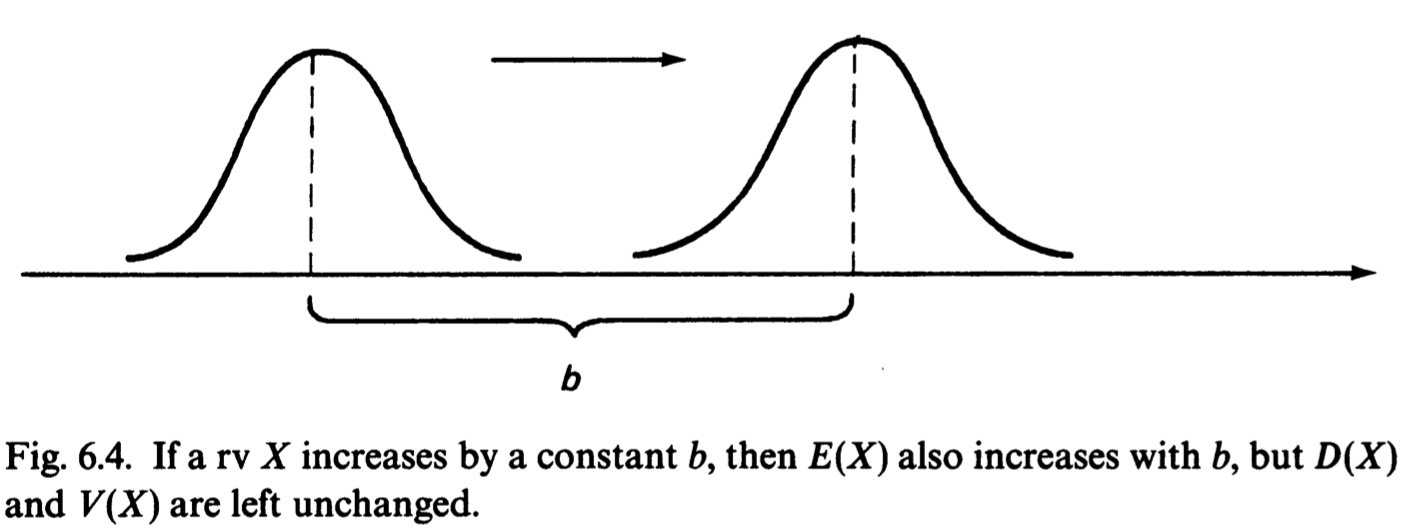
\includegraphics[scale=0.35]{change-move-distribution} \par}

\subsubsection{Standardized rv}

If $X$ is a rv with expectation $m$ and standard deviation $\sigma$, we call $Y = \frac{(X - m)}{\sigma}$ a \textbf{standardized} rv.

\begin{equation}
    E(Y) = E[(X - m) / \sigma] = \frac{1}{\sigma} E(X) - \frac{m}{\sigma} = 0
\end{equation}
\begin{equation}
    V(Y) = \frac{1}{\sigma^2} V(X) = 1
\end{equation}

Hence a standardized rv has mean 0 and variance 1.

\subsubsection{Error}

\textbf{Systematic error} is the difference between the mean of the measured value and the true value. \textbf{Random error} is the difference between the measured value and its mean.

It is important to distinguish between \textbf{accuracy} and \textbf{precision}. By high accuracy we mean good agreement between measured value and true value; by high precision we mean small random error.

\end{multicols*}
\end{document}
